\documentclass{resume} % Use the custom resume.cls style
\usepackage[utf8]{inputenc}
\usepackage[T2A]{fontenc}
\usepackage{textcomp}
\usepackage[russian]{babel}
\usepackage{hyperref}
\hypersetup{
    hidelinks
}
\usepackage{tikz}
\usepackage{graphicx}

\usepackage[left=0.4 in,top=0.4in,right=0.4 in,bottom=0.4in]{geometry} % Document margins
\newcommand{\tab}[1]{\hspace{.2667\textwidth}\rlap{#1}} 
\newcommand{\itab}[1]{\hspace{0em}\rlap{#1}}


\name{Протасов Александр} 
\address{+7(985) 166-07-77 $|$ Москва}
\address{\href{mailto:protasov.alexander@icloud.com}{\underline {protasov.alexander@icloud.com}} $|$ \href{https://t.me/its_pav}{\underline {t.me/its\_pav}} $|$ \href{https://github.com/tymillnyc} {\underline {git: tymillnyc}}}

\begin{document}

\begin{tikzpicture}[remember picture,overlay]
  \node[anchor=north east,inner sep=0pt,xshift=-10mm,yshift=-5mm] at (current page.north east) {
    \begin{tikzpicture}
      \clip[rounded corners=10pt] (0,0) rectangle (2.5cm,2.5cm); % Задаём размеры прямоугольника, равные размеру изображения
      \node[inner sep=0pt] at (2.75cm,2.5cm) { % Позиционирование изображения в центре обрезанного прямоугольника
        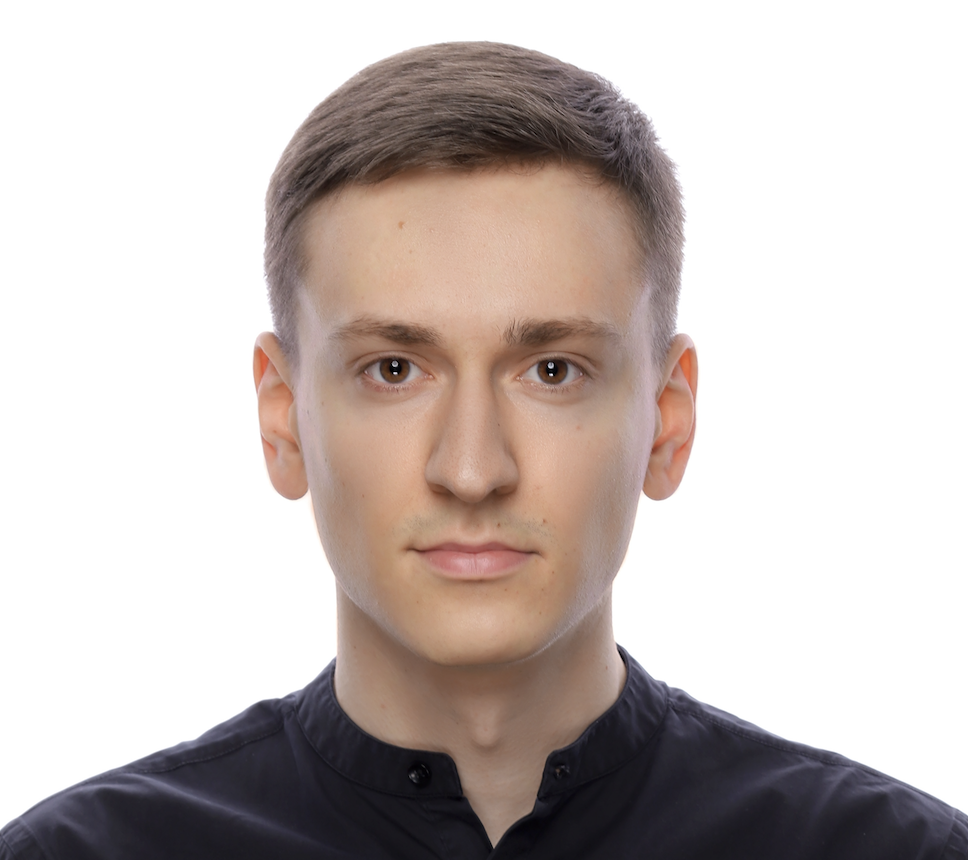
\includegraphics[width=3cm]{ind2.jpg} % Подставьте своё изображение
      };
      \draw[rounded corners=10pt, line width=1pt, draw=gray] (0,0) rectangle (2.5cm,2.5cm); % Добавляем рамку вокруг области обрезки
\end{tikzpicture}
};
\end{tikzpicture}



%----------------------------------------------------------------------------------------
%	OBJECTIVE
%----------------------------------------------------------------------------------------

\begin{rSection}{О себе}

{Окончил бакалавриат с отличием. Ищу full-time работу или стажировку.} \\
{Интересуюсь backend-разработкой, функциональным программированием.}  \\
{\href{https://github.com/tymillnyc/aboutme/blob/main/proofs/codebattle_ydx.pdf} {\underline{Участник}} турнира \textquotedbl{}Intern Codebattle\textquotedbl{} от Яндекса.} 


\end{rSection}
%----------------------------------------------------------------------------------------
%	EDUCATION SECTION
%----------------------------------------------------------------------------------------

\begin{rSection}{Образование}

{\bf Московский государственный университет им. Ломоносова}  \hfill {2019 - 2023} \\
{ Бакалавр. Факультет вычислительной математики и кибернетики, кафедра алгоритмических языков.} \\ \\
{\bf Московский государственный университет им. Ломоносова}  \hfill {2023 - 2025} \\
{ Студент-магистр. Факультет вычислительной математики и кибернетики, направление "Интеллектуальные системы".} 

\end{rSection}

%----------------------------------------------------------------------------------------
% TECHINICAL STRENGTHS	
%----------------------------------------------------------------------------------------
\begin{rSection}{Навыки}
\begin{itemize}
  \item Java Core
  \item SQL, Git, Docker
  \item Python (NLP), C++, C
\end{itemize}
\end{rSection}


%----------------------------------------------------------------------------------------
%	WORK EXPERIENCE SECTION
%----------------------------------------------------------------------------------------

\begin{rSection}{Проекты}
\begin{itemize}
\item {Классификация веб-страниц на основе текстового содержимого с помощью языковой модели BERT и реализация графического интерфейса к решаемой задаче, Python, PyQt5. \href{https://github.com/tymillnyc/diploma} {\underline {(Ссылка)}}}
\item {Разработка интерпретатора модельного языка программирования, C++. \href{https://github.com/tymillnyc/PLInterpreter} {\underline {(Ссылка)}}}
\item {Алгоритм построения детерминированного конечного автомата по регулярному выражению, С++. \href{https://github.com/tymillnyc/re2dfa} {\underline {(Ссылка)}}} 
\item {Интерактивный командный интерпретатор, C. \href{https://github.com/tymillnyc/myshell} {\underline {(Ссылка)}}} 
\item {Игра \textquotedbl{}Змейка\textquotedbl{}, Haskell, Sqlite. \href{https://github.com/tymillnyc/chervyak} {\underline {(Ссылка)}}} 
\item {Алгоритм построения регулярной грамматики по конечному автомату, Lisp. \href{https://github.com/tymillnyc/dfa2reggram} {\underline {(Ссылка)}}} 
\item {Расчет экстремума функции методом генетического алгоритма, Pascal. \href{https://github.com/tymillnyc/GeneticAlgorithm} {\underline {(Ссылка)}}} 
\end{itemize}
\end{rSection} 

%----------------------------------------------------------------------------------------


%----------------------------------------------------------------------------------------
%\begin{rSection}{Leadership} 
%\begin{itemize}
%    \item Sample section
%\end{itemize}


%\end{rSection}


\end{document}
